\subsection*{Gran Puente}
"¡Veamos cómo se las arreglan contra el poderoso yo! ¡Y por "yo" me refiero a Gilgamesh! ¡Y por "se las arreglan", quiero decir SE MUEREN!" \\
\indent -- Gilgamesh \\\\
\noindent
Al salir de Cornelia y dirigirse hacia el norte, el grupo se encuentra en los bosques y prados que rodean la ciudad. Después de varias horas de viaje en la tranquilidad de la naturaleza llegan al Gran Puente, que es enorme pero también viejo y quebradizo. Cuando llegan al final del puente, se encuentran con Gilgamesh, que parece haber estado esperándolos. Gilgamesh no es ni bueno ni malo necesariamente. Viaja por el mundo para encontrar armas poderosas para su colección. Garland ha convencido a Gilgamesh para que trabaje para él y le ordena que proteja el puente de cualquier persona que intente cruzar. A cambio, Garland le regaló la legendaria espada Excálibur (o al menos eso es lo que Gilgamesh cree). Al encontrarse con el grupo, Gilgamesh los reconocerá como oponentes potencialmente dignos y desenvainará sus armas.
\pagebreak

\tcbox[left=0pt,top=0pt,right=0pt,bottom=0pt, boxsep=0pt, colframe=accent, sharp corners]{
	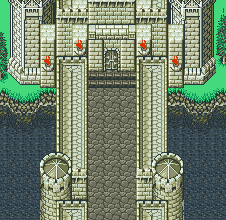
\includegraphics[width=0.96\columnwidth]{./art/maps/bridge.png} 
}

\subsubsection*{Batalla en el Gran Puente}
La batalla contra Gilgamesh tiene lugar al final del puente, como se muestra en el mapa anterior. A continuación se muestran sus características de combate, pero dependiendo del grupo, es posible que tengas que modificar algunos de sus atributos. Cuando los PV de Gilgamesh llegan a 0, no pierde el conocimiento sino que finalmente desenvaina la espada Excálibur para un último ataque. Intenta atacar al miembro más cercano con ella, pero la espada no provoca daño y se destruye inmediatamente. Gilgamesh se da cuenta de que Garland lo ha engañado. Sin otra opción a la vista, decide huír. Como sigue vivo, el grupo puede volver a encontrarse con Gilgamesh en el futuro. Después de derrotar a Gilgamesh, el grupo puede cruzar el puente para llegar al bosque oscuro antes del Santuario del Caos. El bosque está inusualmente silencioso y la mayoría de sus árboles y plantas parecen haber muerto. Es muy probable que los aventureros no lleguen al Santuario antes de la puesta de sol, por lo que probablemente tendrán que pasar la noche en el bosque.

\vspace{0.5cm}

\monster{Gilgamesh}{2}{
\includegraphics[width=0.17\textwidth]{./art/monsters/gilgamesh.png}}
{
 PV: & \hfill 45 & PM: & \hfill 40\\
 FUE: & \hfill 2 & DEF: & \hfill 1 \\
 MAG: & \hfill 0 & RES: & \hfill 0 \\
 AGI: & \hfill 4 & Tamaño: & \hfill M\\
}
{
 \textbf{Arma de Asta}: 1d de daño \hfill \textbf{Botín}: 500 Gil 
 
 \mtech{Garra Letal}{6}{0t}{Único}{Arma}{
 Realiza dos \hyperlink{action}{Ataques} contra el objetivo. Si al menos uno de ellos lo golpea, queda \hyperlink{status}{Inmóvil} por 1 turno. }{\immobile} \mtech{Danza de Espadas}{8}{1t}{3u}{Tú}{Realiza un \hyperlink{action}{Ataque} contra todos los enemigos dentro del área de efecto.}{}
 \mreaction{Poder Crítico}{Cuando tus PV sean menos de 20, recibes \hyperlink{status}{aumFUE} hasta el final de la batalla.} 
}

\pagebreak